\chapter{Generiranje ciljnog programa}

\section{Uvod}

U uvodu je rečeno da ciljni jezik JVM \emph{bytecode}. Java Virtual Machine (JVM) je virtualni stroj koji je prvenstveno
bio namijenjen programskom jeziku Java. Danas postoje razni jezici koji se prevode za JVM. Prednost je prenosivost
takvog koda.

JVM je stogovno orijentirane arhitekture tj. za izvođenje svih operacija se koristi stog. Također postoje 
registri iz kojih se mogu čitati i spremati podaci --- svakoj deklariranoj varijabli je dodijeljen jedan registar, a
indeks registra se određuje po redoslijedu deklariranja varijabli (unutar jedne funkcije tj. metode). 

Naš jezik nije objektno orijentiran jezik, a JVM je prvenstveno bio namijenjen objektno orijentiranoj Javi. Stoga
se svi naši izvorni programi prevode u razred \texttt{Program}, a deklarirane funkcije su zapravo javne metode
tog razreda. Evo primjera jednog programa napisanog u JVM \emph{bytecodeu}:

\lstinputlisting{primjer-bytecode.txt}

Vidimo da se radi o razredu \texttt{Program} koji nasljeđuje \texttt{Object} (takvo je pravilo u Javi)
i da taj razred ima jednu metodu \texttt{main} koja vraća \texttt{int} i ne prima nikakve argumente.

Naredba u liniji 4 stavlja na stog konstantu 10 i nakon toga (linija 5) vrh stoga (konstanta 10) sprema u registar 1.
To su naredbe \texttt{iconst} i \texttt{istore}, a prefix \texttt{i} označava da se radi o cjelobrojnom tipu podataka.

Linije 8 i 9 stave sadržaj registara 1 i 2 na stog. A u liniji 10 se poziva naredba \texttt{iadd} koja
s vrha stoga uzme dva elementa, zbroji ih, i rezultat pospremi na vrh stoga. Taj rezultat koji se sada
nalazi na vrhu stoga se s naredbom \texttt{istore} (linija 11) pospremi u registar 3.

Primjer izvornog koda koji bi se preveo u takav \emph{bytecode} je:

\lstinputlisting[language=C]{primjer-bytecode1.c}

Detaljne specifikacije o JVM bytecode je moguće naći u \cite{jvm}.

\section{Implementacija}

Generiranje nije u potpunosti implementirano. Dio koji je implementiran je implementiran unutar semantičke analize.

Implementirana je deklaracija varijabli i funkcija, obrada izraza (što uključuje i poziv funkcija), vraćanje vrijednosti i
\texttt{ if(expr) \{ ... \} } grananje za demonstraciju kontrole toka.

Kako je JVM stogovno orijentiran, a u sintaksnom stablu je pravilno očuvana prednost operatora, onda je
generiranje koda za izraze bilo jednostavno za ostvariti pomoću rekurzije. 

Također nije u potpunosti implementiran rad s tipovima podataka zbog nekih poteškoća i osobina JVM-a. Pa se u većini
slučajeva kao prefiks koji označava tip podataka koristi \texttt{i} tj. cjelobrojni tip.
\pagebreak
\section{Primjer izvođenja}

Pogledajmo prvo jednostavan primjer gdje su dani samo izrazi bez kontrole toka.

\lstinputlisting[language=C]{primjer-bytecode2.c}

\begin{figure}[H]
  \centering
    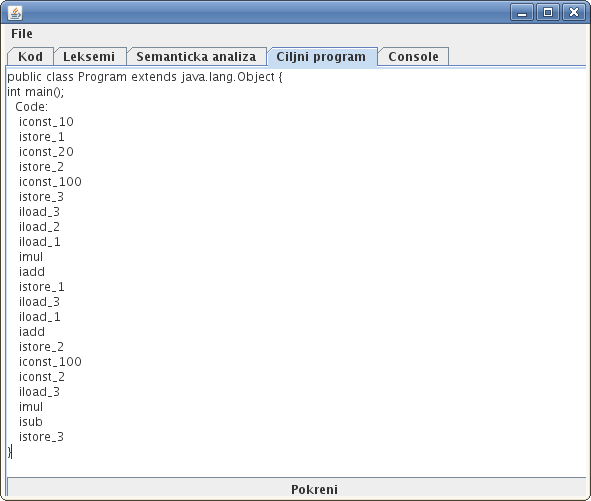
\includegraphics[width=13cm]{primjer-generiranje2}
  \caption{Primjer prevođenja jednostavnog programa}
\end{figure}

U drugom primjeru koristimo "if grananje" i poziv funkcije.

\lstinputlisting[language=C]{primjer-bytecode3.c}

\begin{figure}[H]
  \centering
    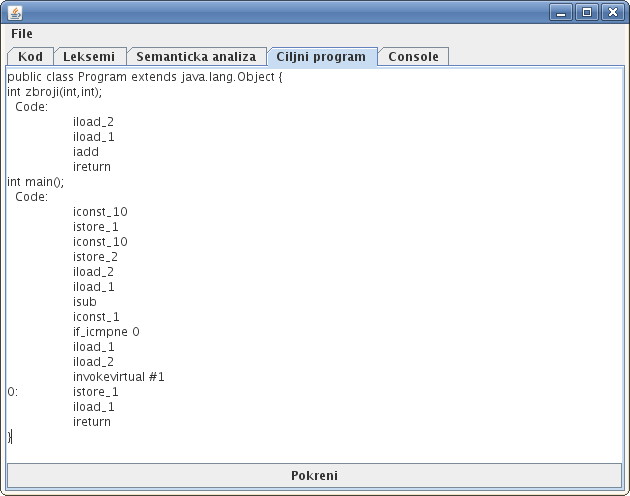
\includegraphics[width=13cm]{primjer-bytecode3}
  \caption{Primjer prevođenja}
\end{figure}

